\documentclass{beamer}
\usepackage[utf8]{inputenc}
\usepackage[T1]{fontenc}
\usepackage{lipsum, lmodern}
\usepackage[scaled=.95]{helvet}% helvetica as the origin of arial
\usepackage[helvet]{sfmath}    % for the mathematical enviroments
\usepackage{graphicx}
\usepackage{multimedia}% for add a movie
\usepackage{hyperref}
\usepackage{media9} %for movie : new try
\renewcommand{\familydefault}{\sfdefault}

%% ETH beamer theme
% Options: [default]
%   itemsblack/[itemsblue]: change color of bullets etc. to black/blue in itemize style environments
%   [titlesblack]/titlesblue: change color of frame titles/subtitles to black/blue
% \usetheme[itemsblack,titlesblack]{eth}
\usetheme{eth}

%% Theme uses ETH blue color by default. Can be changed to any color using this command: 
% \setbeamercolor{structure}{fg=blue}

%% Mandatory variables
\author{Jasmin Fischli, Philipp Göldlin, Julie Veya, Jonathan Burkhard}
\title{Mid-Term Presentation - Beehive Traffic}
\date{\today}

%% Optional variables
 \supervisor{Sattler Torsten} % for one supervisor
%\supervisors{Carol Foote, Jane Smith} % for multiple supervisors
% \projecttype{Master's Thesis}

\begin{document}
\frame{\maketitle}
\begin{frame}{Table of contents}{}
	\tableofcontents
\end{frame}

%Camera support
\section{GoPro support}
\begin{frame}{GoPro support}
\begin{itemize}
\item to have the same view each time
\end{itemize}
\begin{figure}
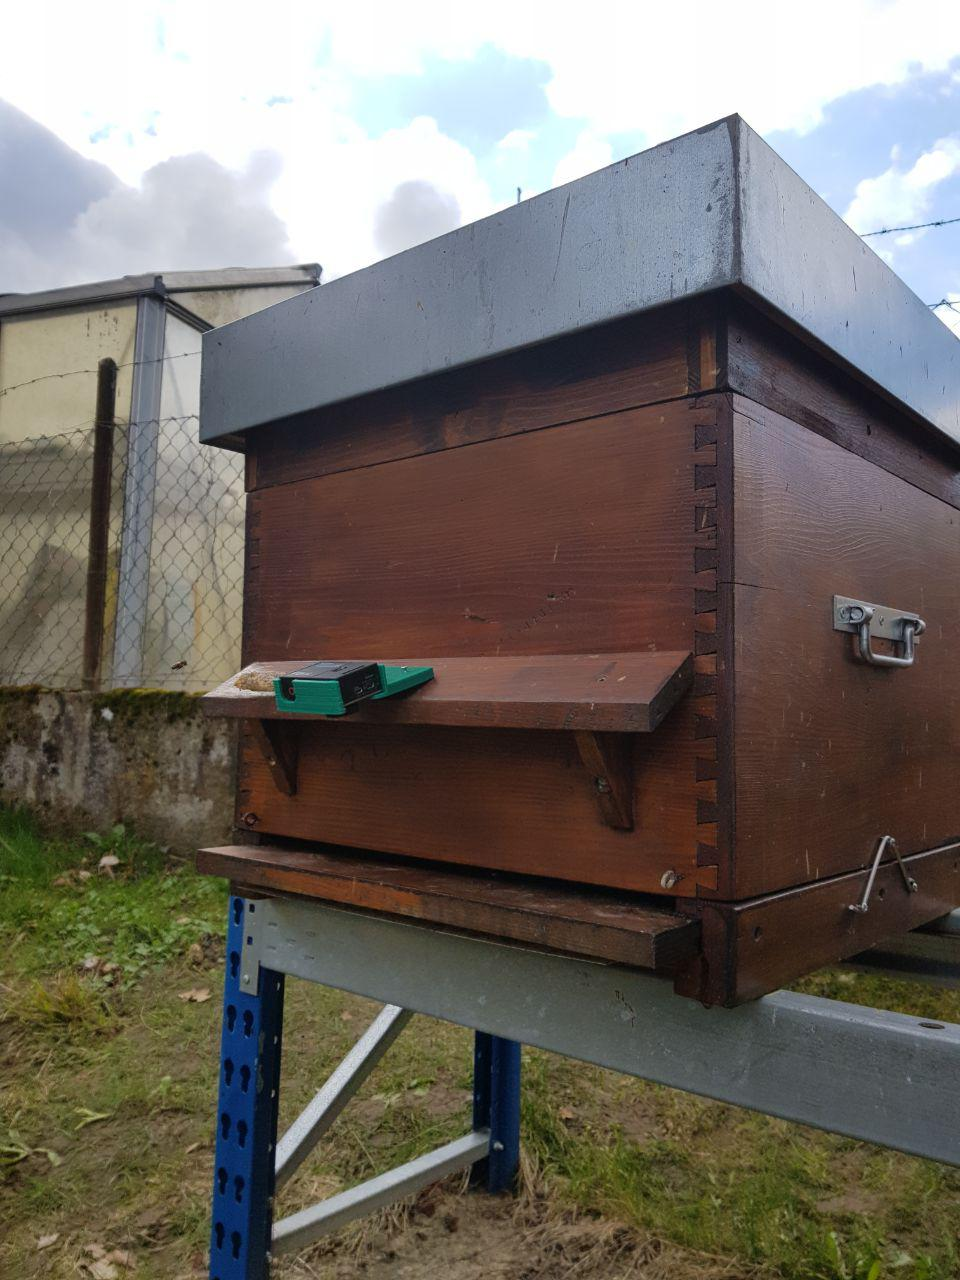
\includegraphics[scale=0.25]{pictures/photoSupport}
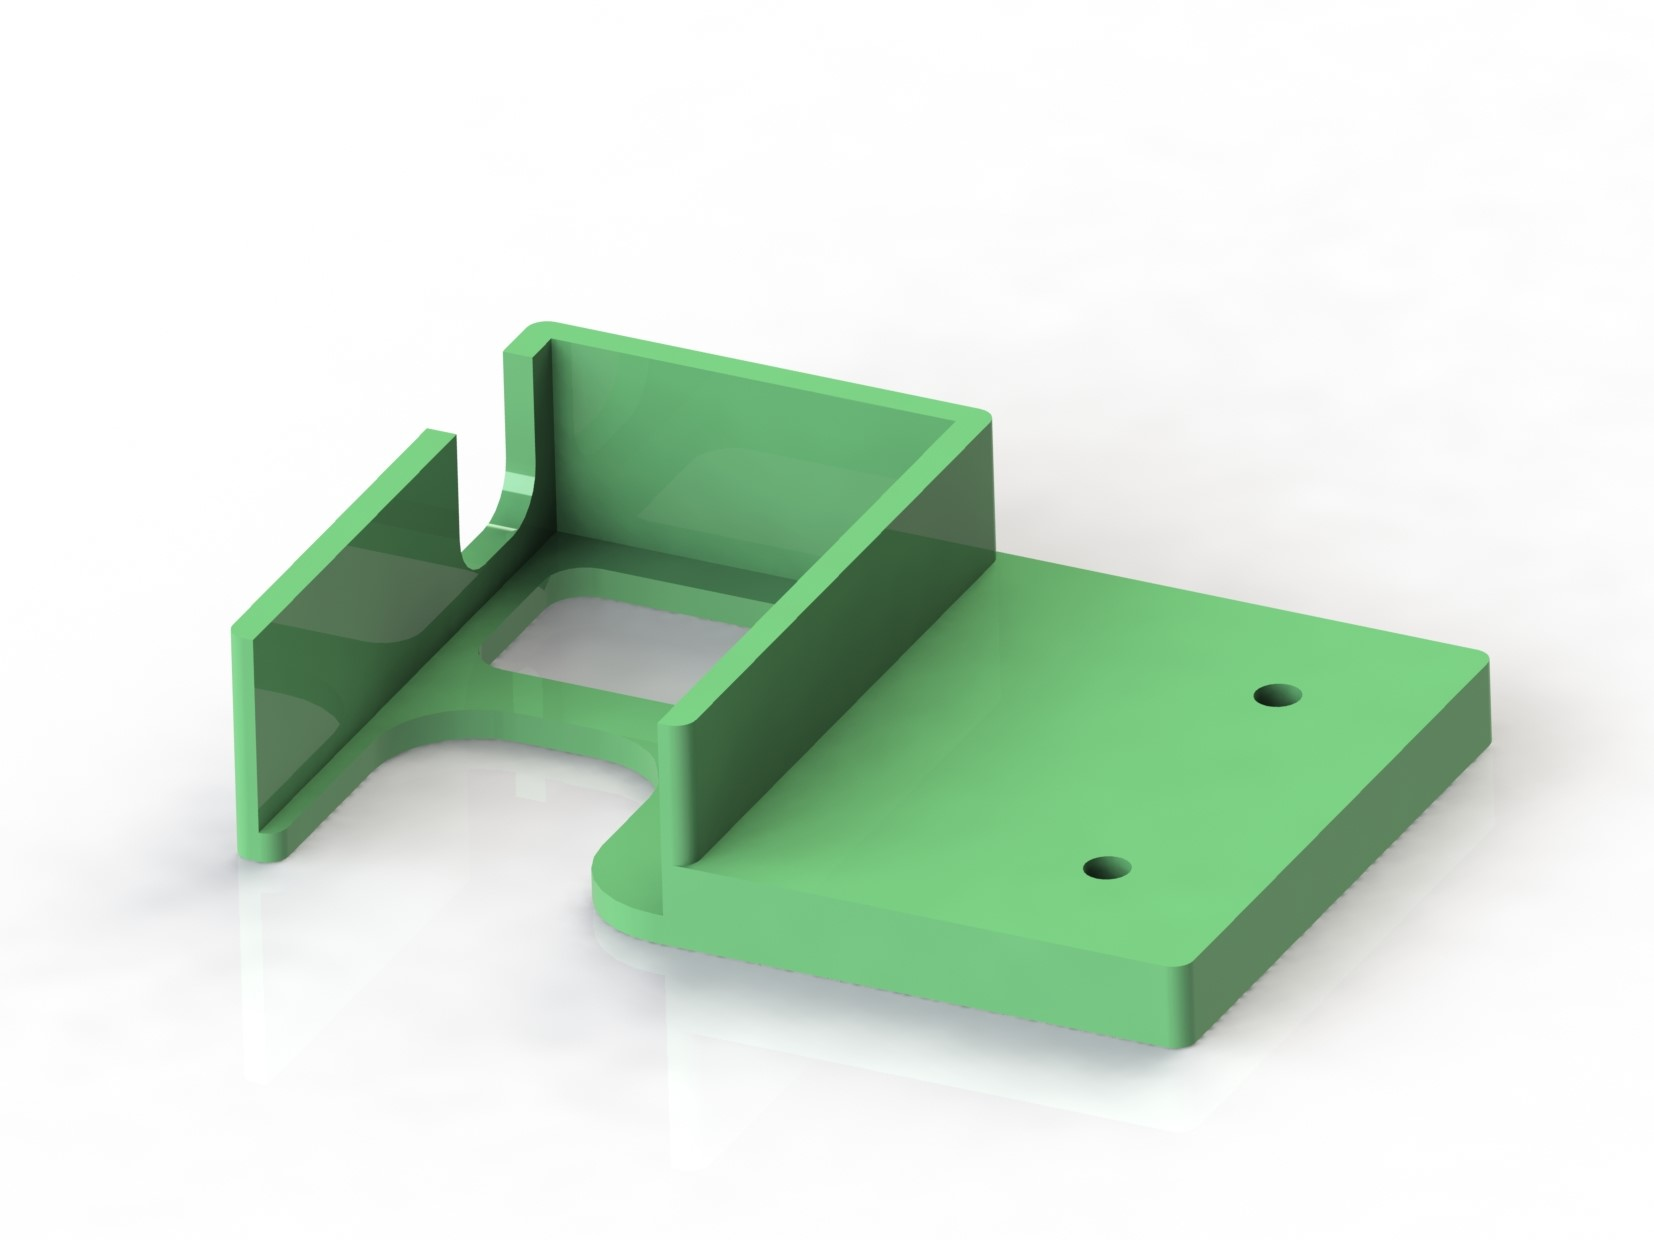
\includegraphics[scale=0.15]{pictures/sup}
\caption{Support of the GoPro in our hive}
\end{figure}
\end{frame}

%slide with a short movie

\begin{frame}{Example of the view with this support}

\begin{figure}
\includegraphics[scale=0.07]{pictures/views}
\caption{View from the support}
\end{figure}
%\movie[label=cells,width=4cm,height=3cm,poster,showcontrols,duration=5s]{}{GOPR1345.MP4}
\end{frame}

\section{Calibration}
\begin{frame}{Calibration}
\begin{figure}
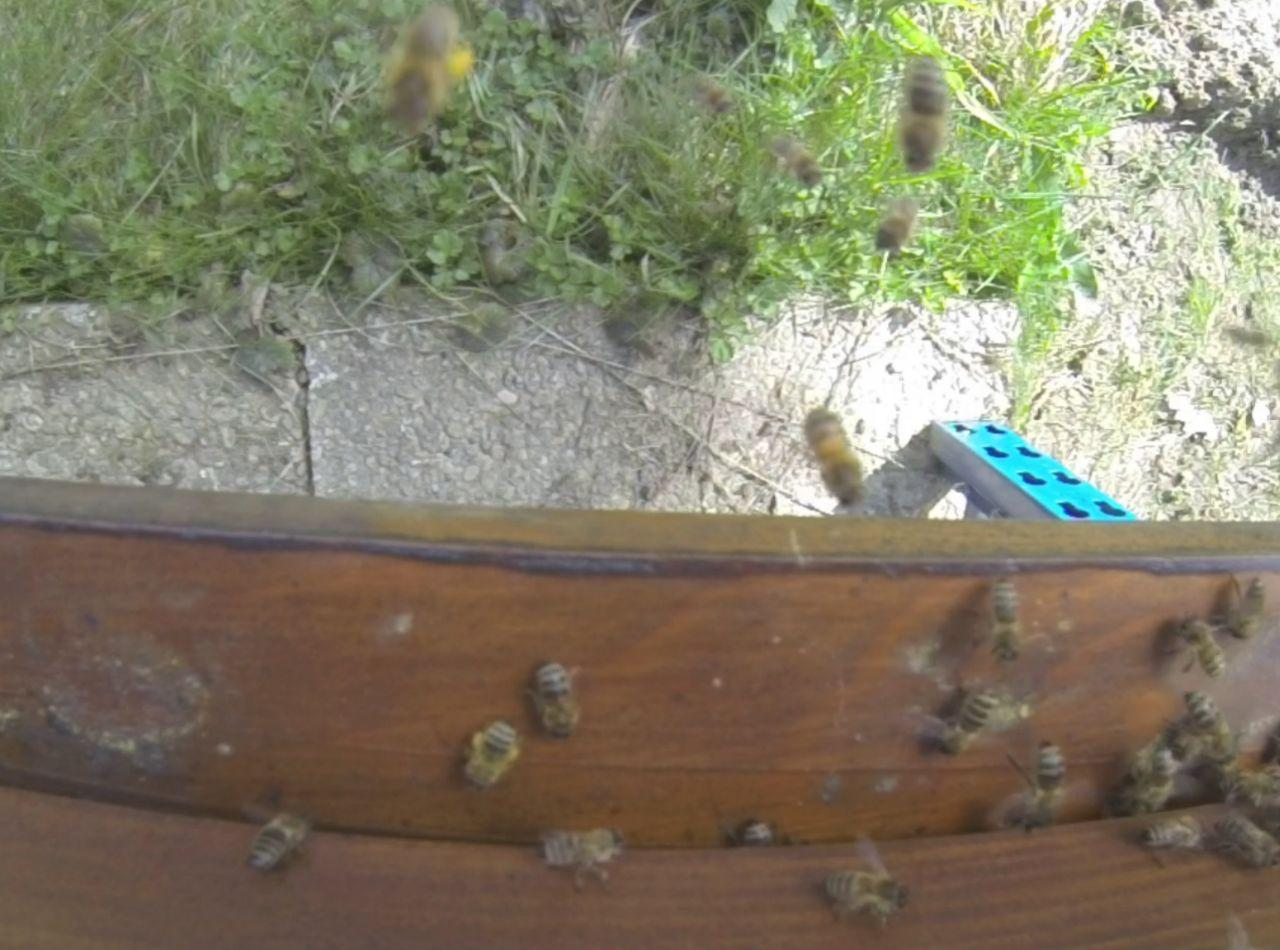
\includegraphics[scale=0.33]{pictures/Dist}
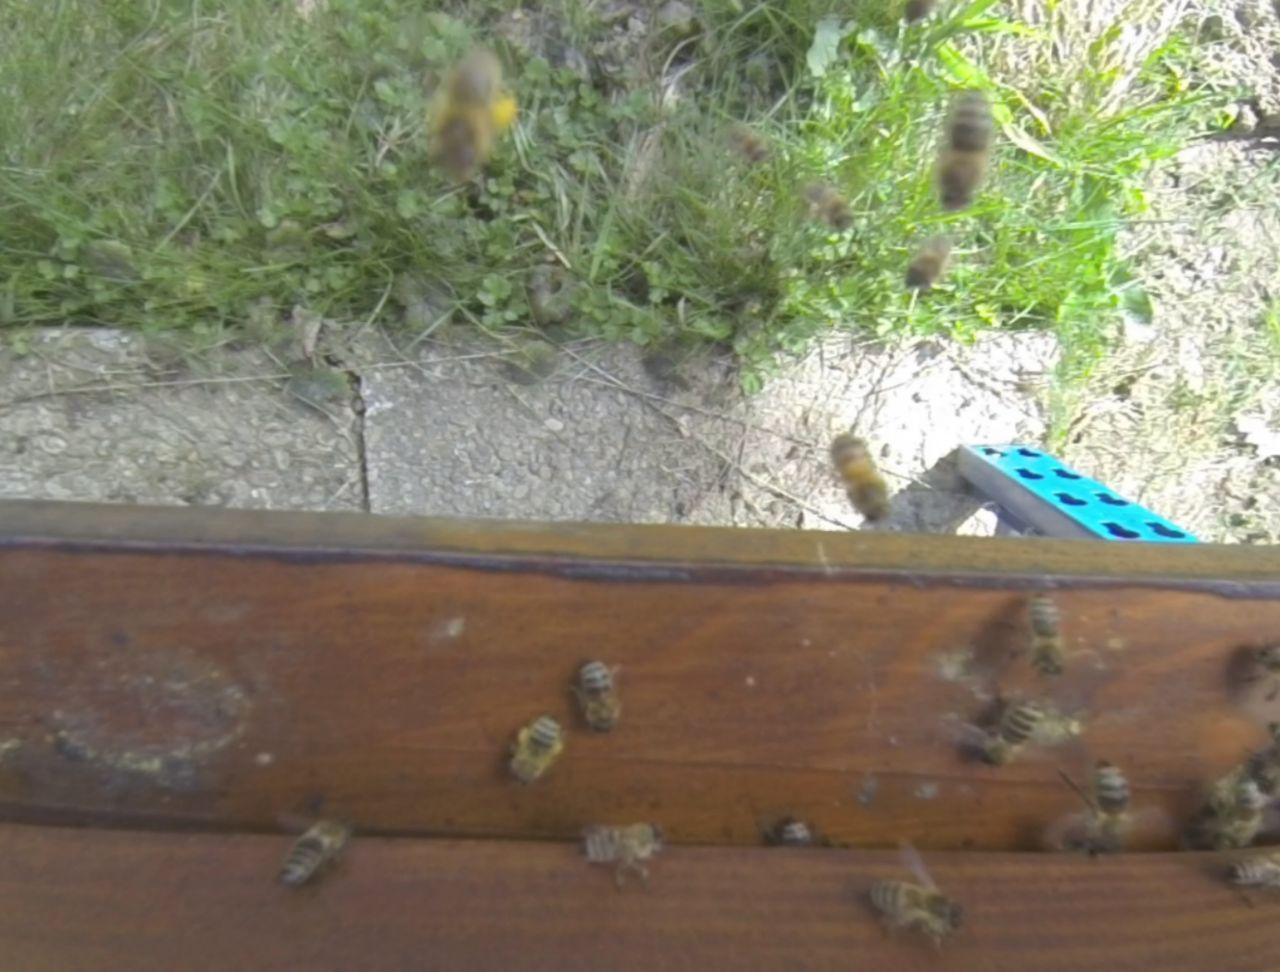
\includegraphics[scale=0.33]{pictures/Calib}
\caption{Left : frame from the gopro, right : frame after calibration}
\end{figure}
\end{frame}

\section{Background subtraction}
\begin{frame}{Background subtraction}
\begin{figure}
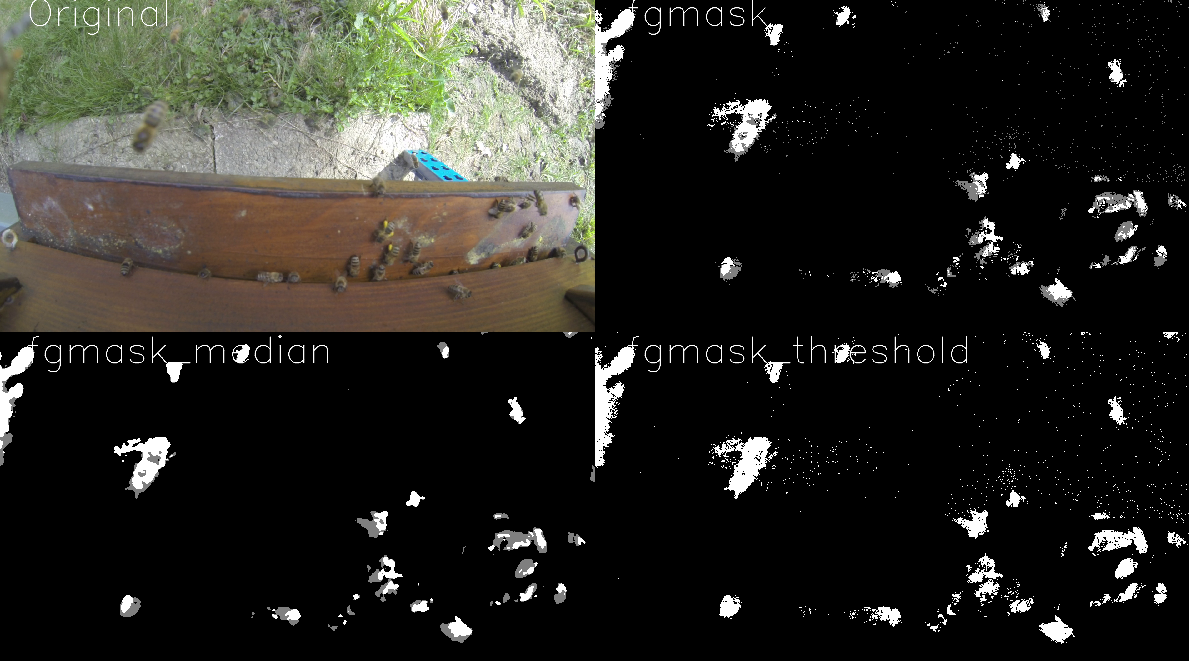
\includegraphics[scale=0.23]{pictures/backg2}
\caption{Original picture, background subtraction, median mask, threshold mask}
\end{figure}
\end{frame}

\section{Bee recognition}
\begin{frame}{Bee recognition}

\centering 
\url{https://www.youtube.com/watch?v=ReSonvV2y0M&feature=youtu.be}
\end{frame}

\section{Which are our next steps?}
\begin{frame}{Which are our next steps?}
\begin{itemize}
\item Enhancement through color histograms, SIFT, grabcut
\item Tracking the bees
\item Count incoming and outgoing bees
\end{itemize}
\end{frame}

\section{Timetable}
\begin{frame}{Timetable}
\centering
\begin{figure}
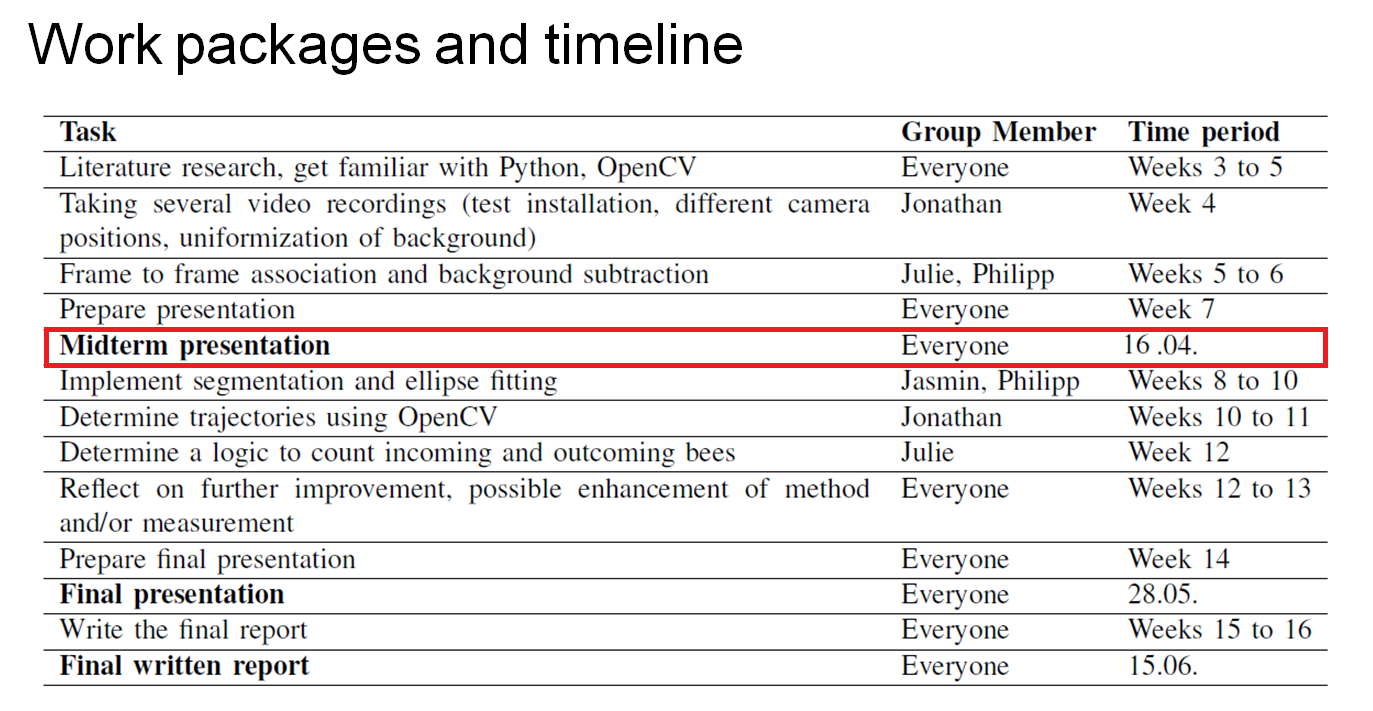
\includegraphics[scale=0.4]{pictures/timeline}
\end{figure}
\end{frame}

\begin{frame}{}
\centering
\Huge{Thank you for your attention !}
\end{frame}



\end{document}
%Document end *************************************************

\section{Introduction}
\subsection{One subsection}
\begin{frame}{Itemize}
\begin{itemize}
\item Here you can see an itemization
\begin{itemize}
\item It has items
\begin{itemize}
\item The items are below each other
\end{itemize}
\end{itemize}
\end{itemize}
\end{frame}

\begin{frame}{Enumerate}
\begin{enumerate}
\item Here you can see an enumeration
\item It has items
\item The items are numbered
\end{enumerate}
\[
	f(x)=\sum_{i=0}^\infty \frac{f^{(i)}(x_0)}{i!}(x-x_0)^i
\]
\end{frame}

\subsection{New Subsection}
\begin{frame}{Theorems and environments}
\begin{theorem}[Sample theorem]
This presentation is essentially useless.
\end{theorem}
\begin{proof}
This proof is essentially incorrect.
\end{proof}
\end{frame}

\begin{frame}{Example slide with Title}
\begin{example}
Major problem.
\end{example}
\begin{solution}
Minor nuisance.
\end{solution}
\end{frame}

\begin{frame}[plain]{Plain frame with title}
\lipsum[1]
\end{frame}


